\documentclass[12pt]{article}
\usepackage{mathptmx}
\usepackage[margin=1in]{geometry} 
\usepackage{fancyhdr}
\usepackage{graphicx}
\usepackage{setspace}
\usepackage{indentfirst}


\renewcommand{\baselinestretch}{1.5} 

\begin{document}
\pagestyle{fancy}
\lhead{COMP90015}\chead{Assignment 1}\rhead{Semester 1, 2021}

\thispagestyle{empty}
\begin{center}
\Large\sc{COMP90015 Distributed Systems}
\end{center}

\begin{center}
\Large\bf{Multi-threaded Dictionary Server}
\end{center}

\begin{center}
Name: JIAQI WANG \ \ ID: 908406
\end{center}

\section{Introduction}
With the power of internet, nowadays users can have access to services anywhere from the world. In this context, a distributed system is superior to a single machine to serve these needs. Distributed systems have advantages such as functional separation, inherent distribution, power imbalance and load variation, reliability and economies.

In this assignment, I will explore the distributed system by designing and implementing a multi-threaded dictionary using Java to allow concurrent clients searching the meanings of a word, adding a new word, and removing an exisiting word.

\subsection{Architecture}
From the top, the system will follow client-server architecture. A single multi-threaded sever is running and listening for connections from clients. Concurrency in the server is carefully handled by the use of ConcurrentHashMap.

\subsection{Interaction}
All communication will take place via TCP sockets. In addition, JSON is used to be the message exchange protocol.

\subsection{Failure Model}
Errors handling in server side includes printing stack-trace messages and assigning default values. In client side it includes showing dialog windows and requiring user to fix the inputs.

\newpage
\section{System Components}
The server program, the client program and the client GUI are \texttt{Server.java}, \texttt{Client.java} and \texttt{ClientWindow} correspondingly.

\subsection{\texttt{server.java}}
The server is invoked through the \texttt{main()}. The port number is read from \texttt{args[0]}. In case when any error occurred, the default port number 3005 will be assigned. The dictionary is a \texttt{ConcurrentHashMap} instance, constructed using the provided dictionary JSON file. Then the server tries to instantiate a \texttt{ServerSocket} with the port number. In the while loop, the \texttt{serverSocket} blocks until a connect is accepted. It passes the client's socket to a new thread for processing all following requests. The loop then repeats listening connection and so on. 

The \texttt{serveClient()} handles requests from a client. It first prints which client is connect. Then it tries to \texttt{readUTF()} from \texttt{DataInputStream} in a while loop. A request is a JSON String with internal structure \{command, word, meaning\}. Once a request message is received, it is deserialized and processed accordingly. The results and errors are put into an \texttt{ObjectNode}, which is serialized at the end and written in \texttt{DataOutputStream}. When an \texttt{EOFException} is thrown in reading input stream, it means a client has closed GUI window, so the server prints a message saying that the client is disconnected.

\subsection{\texttt{Client.java}}
This \texttt{Client} class has constructor which takes two arguments ip and port and creates corresponding socket and data streams. The method \texttt{action()} is serializing a command sent to the server and returning an deserialized \texttt{ObjectNode} result.

\subsection{\texttt{ClientWindow}}
\texttt{ClientWindow()} creates a frame and a connection panel is shown by \texttt{connect()}. After a user input IP and port for connection, \texttt{initialize()} removes the connection panel and adds a tabbed content panel for different functionalities.

\newpage
\section{Class Design}
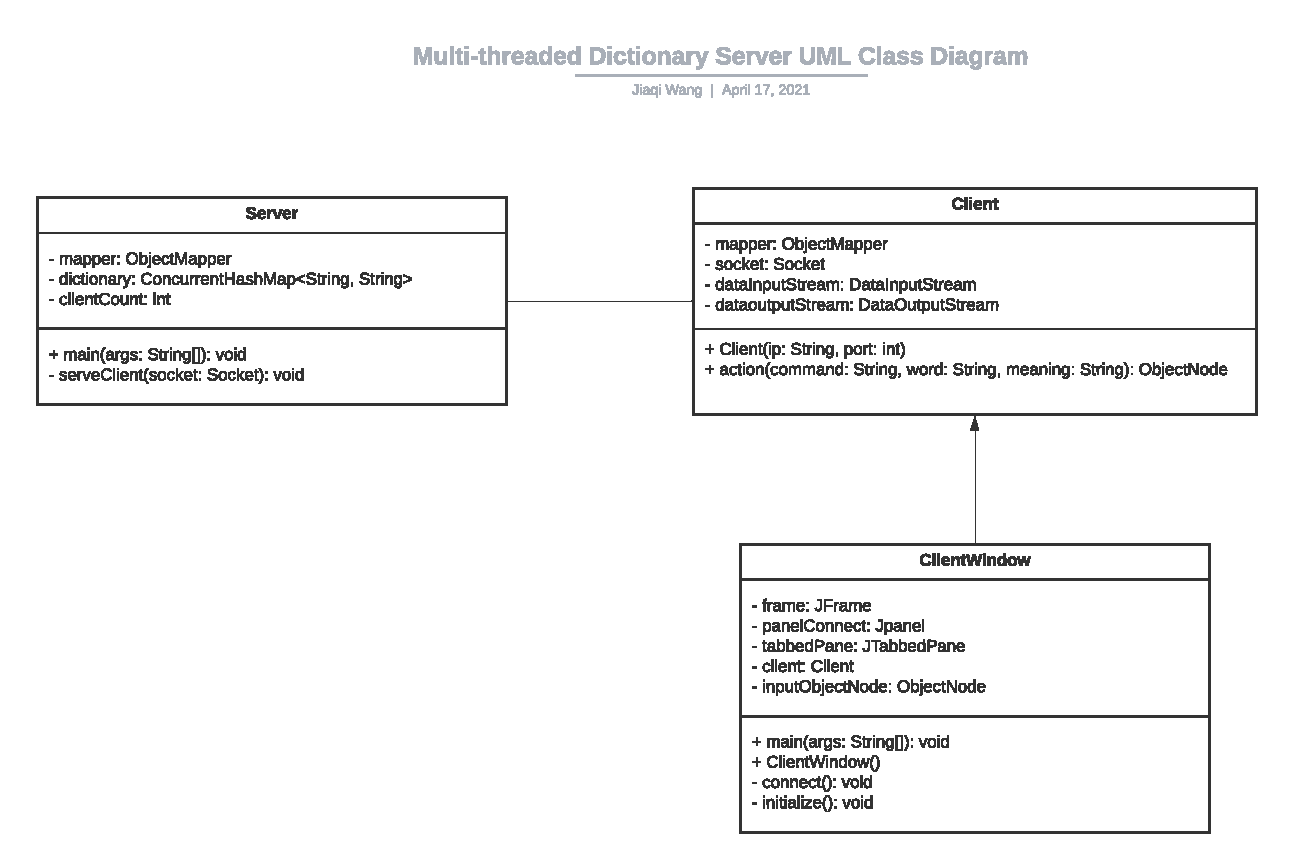
\includegraphics[scale=0.65]{Multi-threaded Dictionary Server UML Class Diagram}

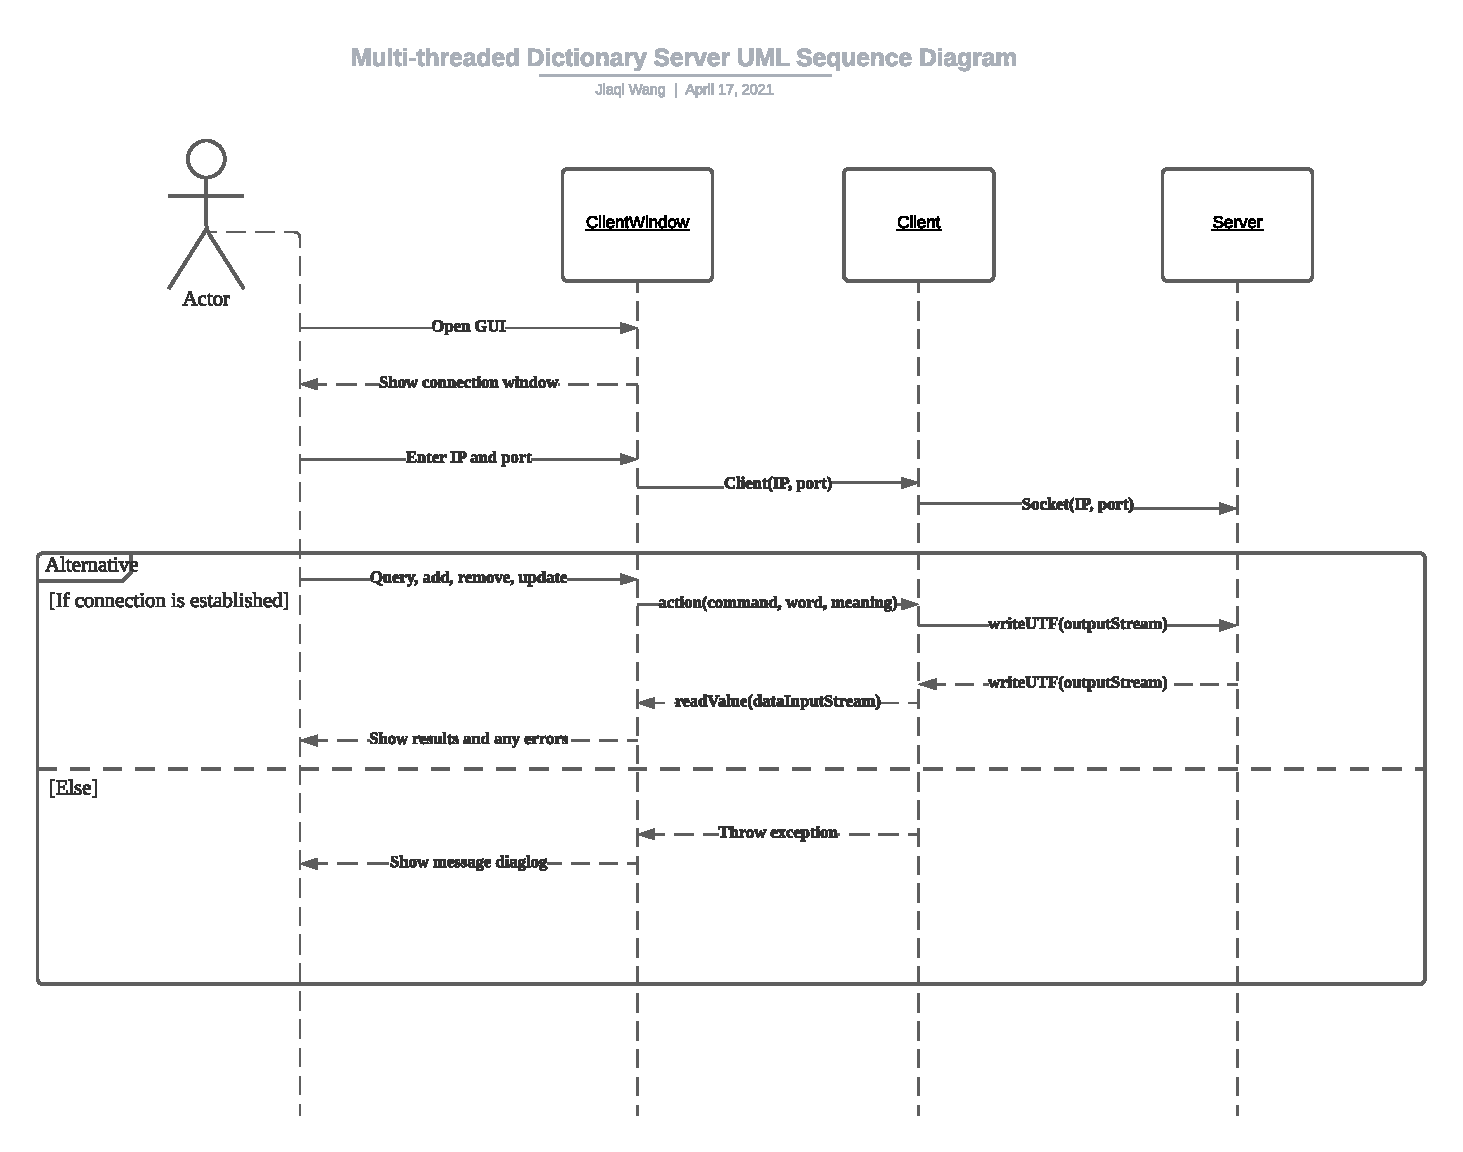
\includegraphics[scale=0.6]{Multi-threaded Dictionary Server UML Sequence Diagram}
\newpage

\section{Evaluation}
The design choices might have following advantages and disadvantages.
\begin{itemize}
\item For the thread architecture, a thread-per-connection approach is chosen since it is more intuitively to have one thread serves one client and requests from one client at a time can be easily handled by one thread in this dictionary application. However, the client might need to wait for the thread-creation comparing to worker-pool architecture.
\item TCP sockets provide reliable communication since it has taken care of all kinds of network issues in the transport layer. But it's speed is slower than UDP. The message passed between the server and the clients are all tiny, so it doesn't impact much in this dictionary application.
\item The message exchange protocol JSON has advantages of being light-weighted and human-readable. But it requires external library Jackson to process, which is not very portable and might brings performance issues.
\end{itemize}

\subsection{Excellence Elements}
\begin{itemize}
\item Notification of errors are shown in a dialog window, which really help user to understand what went wrong.
\item A user can use GUI to enter IP address and port for the server, which makes the GUI more user-friendly. If connection is refused for specific IP and port, an message dialog window will appear. A user checks to see the cause and then re-connects again.
\end{itemize}
\subsection{Creativity Elements}
\begin{itemize}
\item A tabbed pane is designed in client GUI to seperate different functionalities. It can effectively prevent any operation mistake and make GUI more intuitive. 
\item In the server, a \texttt{ClientCount} is kept. It helps to keep track of how many clients have connected and identify which client is currently connecting and disconnecting.
\end{itemize}
\end{document}